\chapter{Analisi dati}
Gli obiettivi principali di queste analisi sono:
\begin{itemize}
    \item Mostrare delle statistiche generali sul dust e sul comportamento degli indirizzi che lo ricevono;
    \item Descrivere alcuni pattern interessanti che sono stati trovati e che potrebbero rappresentare casi di Dust Attack.
\end{itemize}
\section{Statistiche generali}
I dati analizzati comprendono le transazioni dal \textbf{3 Gennaio 2009} al \textbf{10 Agosto 2017}.
Come spiegato precedentemento il primo obiettivo è quello di presentare statistiche generali sull'uso del dust, per questo motivo il primo compito eseguito è stato il filtraggio di tutte le transazioni dust. Le transazioni dust sono quelle transazioni che contengono almeno un input dust o almeno un output dust.
\begin{mdframed}
 infos:inputs:118890,\textbf{99},2;118902,9987098901,2 \checkmark\\
 infos:21482214,984902,114569039,1;21482868,\textbf{1},73028796,240:outputs \checkmark\\
 infos:118925,9963398109,121409,0:118926,9962398010,2 \textbf{x}
\end{mdframed}
Le prime due transazioni sono considerate nelle analisi successive, l'ultima invece è stata ignorata perchè di poco interesse ai fini dello studio del Dust Attack.\\
Le transazioni totali sono 245 410 083 mentre le transazioni dust sono 2 114 335, questo significa che il dust è presente solo nello 0.8\% delle transazioni totali; inoltre come riportato in\cite{dustAnalisi} 1 705 560 creano dust mentre solo 429 544 lo consumano. Da questi due ultimi risultati possiamo dedurre che ci sono transazioni in cui il dust è presente sia negli input che negli output.\\\\
Il passaggio successivo è stato il filtraggio delle transazioni generate da Satoshi Dice. Satoshi Dice\cite{SD} è un noto servizio di gambling, nato nell'Aprile 2012, che usa il dust per comunicare ai giocatori perdenti che hanno perso la loro scommessa. Data la notorietà del servizio, risulta molto poco probabile che l'intento sia quello di un Dust Attack.\\
Le transazioni generate da Satoshi Dice sono 1 465 295, ovvero il 69\% delle transazioni dust. Questo significa che i possibili attaccanti sono presenti nel rimanente 31\%, ovvero nelle restanti 649 040 transazioni dust.\\\\
Una volta ottenute tutte e sole le transazioni di interesse ho realizato il seguente istogramma che mostra la distribuzione del numero di input dust e output dust. In entrambi i grafici le colonne rappresentano un gruppo di cinquanta valori.
\begin{figure}[h!]
    \centering
    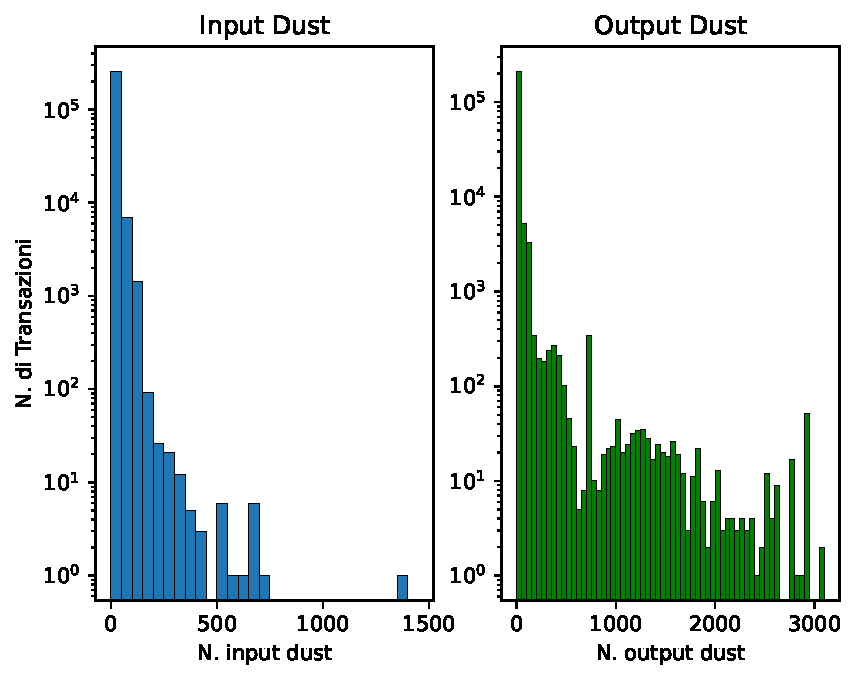
\includegraphics[scale=1]{Grafici/distribuzione_dust.pdf}
    \caption{Distribuzione numero input dust(sinistra) e output dust(destra)}
    \label{fig:dust_distribuzione}
\end{figure}
\FloatBarrier 
Dal primo istogramma possiamo notare come siano molto frequenti le transazioni con un numero di input dust nell'intervallo [1, 50), al contrario le transazioni con un elevato numero di input dust risultano poco usuali.\\
Il secondo grafico mostra come anche in questo caso sia molto frequente avere un numero di output dust nell'intervallo [1, 50). Al contratio del primo istogramma però possiamo notare come siano presenti molte più transazioni con un elevato numero di output dust. Da questi due grafici inoltre possiamo già intuire che molto output dust generato non venga successivamente speso.\\\\ 
Nelle analisi successive viene ignorato il dust generato con script OP\_RETURN. Questa scelta è motivata dal fatto che gli output con questo script non possono essere spesi; chi lo genera sicuramente non sta attuando un Dust Attack.\\
Il grafico seguente mostra la generazione del dust spendibile nel tempo.
\begin{figure}[h!]
    \centering
    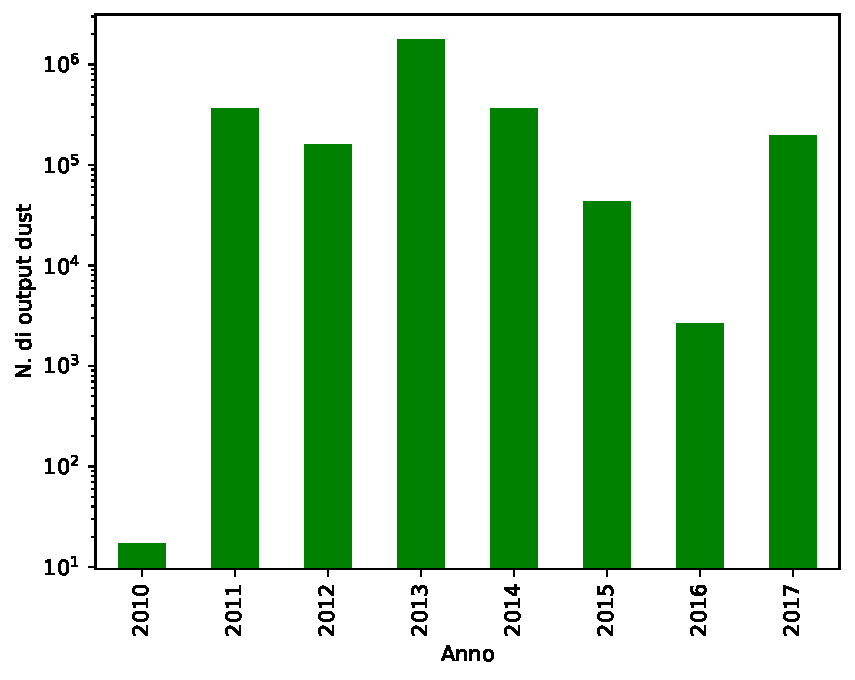
\includegraphics[scale=0.9]{Grafici/dust_created_year.pdf}
    \caption{Creazione dust nel tempo}
    \label{fig:dust_distribuzione}
\end{figure}
\FloatBarrier 
Dall'istogramma notiamo che già dal 2010 sono comparsi i primi output dust, anche se in quantità molto ridotta. Possiamo osservare una rapida salita tra il 2010 e il 2011, solo nel mese di luglio infatti sono stati generati 27 376 output dust, tramite transazioni legate "a catena"; nel paragrafo successivo approfondirò il concetto delle "catene". 
Il picco della generazione del dust lo abbiamo nel 2013, dove sono state trovate diverse catene simili a quella del 2011 ma con una sostanziale differenza che spiegherò successivamente. Dopo il picco del 2013 osserviamo una diminuzione del dust negli anni fino al 2017 dove sembrerebbe esserci una crescita del dust. Bisogna però specificare che la maggior parte del dust generato nel 2017 proviene da due indirizzi: 1Enjoy1C4bYBr3tN4sMKxvvJDqG8NkdR4Z e 1SochiWwFFySPjQoi2biVftXn8NRPCSQC. Questi due noti indirizzi sono comparsi per la prima volta nel 2014, legati alle olimpiadi di Sochi in Russia, 
\begin{figure}[h!]
    \centering
    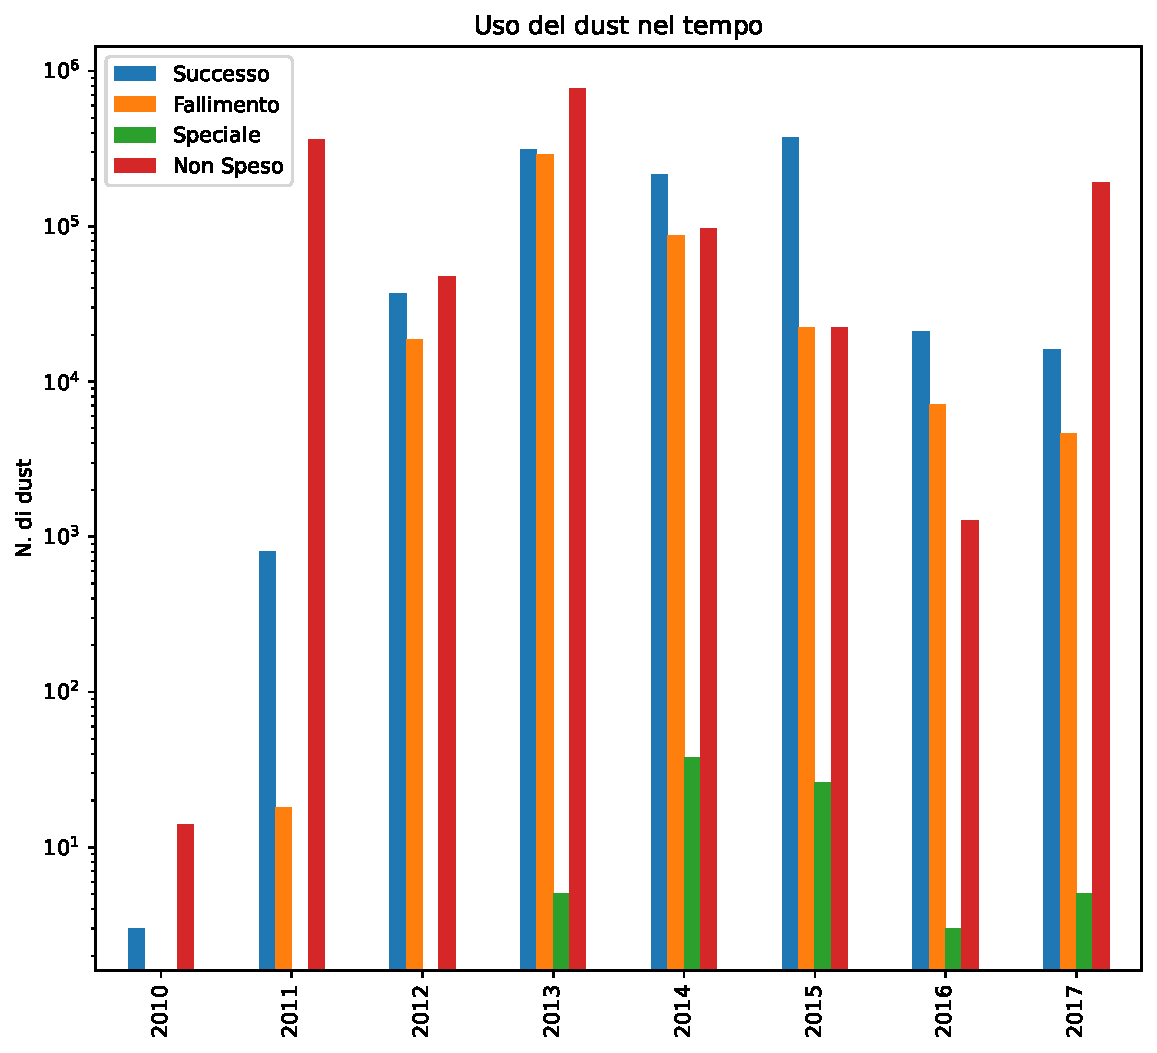
\includegraphics[scale=0.7]{Grafici/uso_del_dust_new.pdf}
    \caption{Uso del dust nel tempo}
    \label{fig:dust_year}
\end{figure}
\FloatBarrier
Il dust generato è stato suddiviso in quattro categorie:
\begin{enumerate}
    \item Successo:
    \item Fallimento:
    \item Speciale:
    \item  Non speso:
\end{enumerate}

\section{Pattern Particolari}
\begin{itemize}
    \item catena dust
    \item tante Tx stesso timestamp stesso tutto
    \item tante Tx breve tempo, tanti output ecc...
\end{itemize}